%%%%%%%%%%%%%%%%%%%%%%%%%%%%%%%%%%%%%%%%%%%%%%%%%%%%%%%%%%%%%%%%%%%%%%%%%%%%%%%
% Copyright (c) 2016-7 Bryce Adelstein Lelbach aka wash <brycelelbach@gmail.com>
%
% Distributed under the Boost Software License, Version 1.0. (See accompanying
% file LICENSE_1_0.txt or copy at http://www.boost.org/LICENSE_1_0.txt)
%%%%%%%%%%%%%%%%%%%%%%%%%%%%%%%%%%%%%%%%%%%%%%%%%%%%%%%%%%%%%%%%%%%%%%%%%%%%%%%

\documentclass[10pt, conference, compsocconf]{IEEEtran}

%%%%%%%%%%%%%%%%%%%%%%%%%%%%%%%%%%%%%%%%%%%%%%%%%%%%%%%%%%%%%%%%%%%%%%%%%%%%%%%

% Hacks to revert the changes IEEEtran makes to table caption styles

\usepackage{etoolbox}

\makeatletter
\patchcmd{\@makecaption}
  {\scshape}
  {}
  {}
  {}
\makeatother

%%%%%%%%%%%%%%%%%%%%%%%%%%%%%%%%%%%%%%%%%%%%%%%%%%%%%%%%%%%%%%%%%%%%%%%%%%%%%%%

%\usepackage{lmodern}
\usepackage{amsmath}
\usepackage{amsfonts}
\usepackage{cite}

% Disable links.
\usepackage[draft]{hyperref}

% Enable links.
%\usepackage[hidelinks]{hyperref}

\usepackage{color}

\usepackage{graphicx}  % \includegraphics
\usepackage{multirow}  % \multicolumn, \multirow
\usepackage{subfig}    % \subfloat

% Place subfigure captions on top
\captionsetup[subfigure]{position=top}

% Make figure labels bold
\captionsetup[figure]{labelfont=bf}

%%%%%%%%%%%%%%%%%%%%%%%%%%%%%%%%%%%%%%%%%%%%%%%%%%%%%%%%%%%%%%%%%%%%%%%%%%%%%%%

% Highlighted source code listings

\definecolor{darkblue}{rgb}{0,0,.6}
\definecolor{darkred}{rgb}{.6,0,0}
\definecolor{darkgreen}{rgb}{0,.6,0}

\usepackage{listings}
\lstloadlanguages{C++}

\lstset{
language=C++,                       % choose the language of the code
basicstyle=\footnotesize\ttfamily,  % the size of the fonts that are used for the
                                    % code
numbers=none,                       % where to put the line-numbers
numberstyle=\tiny,                  % the size of the fonts that are used for the
                                    % line-numbers
stepnumber=1,                       % the step between two line-numbers. If it's
                                    % 1 each line will be numbered
numbersep=5pt,                      % how far the line-numbers are from the code
showspaces=false,                   % show spaces adding particular underscores
showstringspaces=false,             % underline spaces within strings
showtabs=false,                     % show tabs within strings adding particular
                                    % underscores
keywordstyle=\bfseries\lst@ifdisplaystyle\color{blue}\fi, % color of the keywords
commentstyle=\color{darkgreen},     % color of the comments
stringstyle=\color{darkred},        % color of strings
captionpos=b,                       % sets the caption-position to top
tabsize=2,                          % sets default tabsize to 2 spaces
frame=tb,                           % adds a frame around the code
breaklines=true,                    % sets automatic line breaking
breakatwhitespace=false,            % sets if automatic breaks should only happen
                                    % at whitespace
escapechar=\%,                      % toggles between regular LaTeX and listing
belowskip=0.3cm,                    % vspace after listing
morecomment=[s][\bfseries\color{blue}]{struct}{\ },
morecomment=[s][\bfseries\color{blue}]{class}{\ },
morecomment=[s][\bfseries\color{blue}]{public:}{\ },
morecomment=[s][\bfseries\color{blue}]{public}{\ },
morecomment=[s][\bfseries\color{blue}]{protected:}{\ },
morecomment=[s][\bfseries\color{blue}]{private:}{\ },
morecomment=[s][\bfseries\color{black}]{operator+}{\ },
xleftmargin=0.1cm,
}

%%%%%%%%%%%%%%%%%%%%%%%%%%%%%%%%%%%%%%%%%%%%%%%%%%%%%%%%%%%%%%%%%%%%%%%%%%%%%%%

\usepackage{textcomp} % \texttildelow

% Uncomment if using Latin Modern fonts
%\newcommand{\textapprox}{\raisebox{0.5ex}{\texttildelow}}

\newcommand{\textapprox}{\texttildelow}

%%%%%%%%%%%%%%%%%%%%%%%%%%%%%%%%%%%%%%%%%%%%%%%%%%%%%%%%%%%%%%%%%%%%%%%%%%%%%%%

% \thickhline for tables

\usepackage{array}

\makeatletter
\newcommand{\thickhline}{%
    \noalign {\ifnum 0=`}\fi \hrule height 1pt
    \futurelet \reserved@a \@xhline
}
\newcolumntype{"}{@{\hskip\tabcolsep\vrule width 1pt\hskip\tabcolsep}}
\makeatother

%%%%%%%%%%%%%%%%%%%%%%%%%%%%%%%%%%%%%%%%%%%%%%%%%%%%%%%%%%%%%%%%%%%%%%%%%%%%%%%

\usepackage{fixme}

\fxusetheme{color}

\fxsetup{
  status=draft,
  author=,
  layout=inline,
  theme=color
}

% Yellow background and red text for \fxnote

\usepackage{xcolor} % Background highlighting via \colorbox and \textcolor
                    % and \colorlet

\definecolor{fxnote}{rgb}{0.8000,0.0000,0.0000} % Red
\colorlet{fxnotebg}{yellow}

\usepackage{soul}   % \hl

\makeatletter
\renewcommand*\FXLayoutInline[3]{%
  \@fxdocolon {#3}{%
    \@fxuseface {inline}%
    \begingroup
      \sethlcolor{fx#1bg}%
      \color {fx#1}\ignorespaces \hl{#3\@fxcolon #2}%
    \endgroup%
  }%
}
\makeatother

\makeatletter
\renewcommand*\FXLayoutMargin[3]{%
  \marginpar[%
    \@fxdocolon {#3}{%
      \raggedleft%
      \@fxuseface {margin}%
      \begingroup
        \sethlcolor{fx#1bg}%
        \color {fx#1}\ignorespaces \hl{#3\@fxcolon #2}%
      \endgroup%
    }%
  ]{%
    \@fxdocolon {#3}{%
      \raggedright%
      \@fxuseface {margin}%
      \begingroup
        \sethlcolor{fx#1bg}%
        \color {fx#1}\ignorespaces \hl{#3\@fxcolon #2}%
      \endgroup%
    }%
  }%
}
\makeatother

% Yellow background and red text for footnotes

\renewcommand\thefootnote{\colorbox{yellow}{\color{red}\arabic{footnote}}}

%%%%%%%%%%%%%%%%%%%%%%%%%%%%%%%%%%%%%%%%%%%%%%%%%%%%%%%%%%%%%%%%%%%%%%%%%%%%%%%

% Enable for page numbers
%\pagenumbering{arabic}

% Enable for double spacing 
%\linespread{2}

\linespread{0.9}
\renewcommand{\arraystretch}{1.2}

\usepackage{gitinfo2}
\usepackage{datetime}

%%%%%%%%%%%%%%%%%%%%%%%%%%%%%%%%%%%%%%%%%%%%%%%%%%%%%%%%%%%%%%%%%%%%%%%%%%%%%%%

% Force Times New Roman
\usepackage[T1]{fontenc}
\usepackage{times}
\usepackage{mathptmx}
 
%%%%%%%%%%%%%%%%%%%%%%%%%%%%%%%%%%%%%%%%%%%%%%%%%%%%%%%%%%%%%%%%%%%%%%%%%%%%%%%
\begin{document}
\bstctlcite{IEEEexample:BSTcontrol}

\title{Simultaneously Solving Swarms of Small Sparse Systems on SIMD Silicon}

%%%%%%%%%%%%%%%%%%%%%%%%%%%%%%%%%%%%%%%%%%%%%%%%%%%%%%%%%%%%%%%%%%%%%%%%%%%%%%%
\author{\IEEEauthorblockN{Bryce Adelstein Lelbach, Hans Johansen, and Samuel Williams}
\IEEEauthorblockA{Lawrence Berkeley National Laboratory, Computational Research Division\\
brycelelbach@gmail.com, \{hjohansen, swwilliams\}@lbl.gov\\
% Enable for version information.
%{\small Revision \gitAbbrevHash \gitReferences, Built at \currenttime \vspace{1ex} on \today}
}}

\maketitle

% Enable for page numbers
%\thispagestyle{plain}
%\pagestyle{plain}

%%%%%%%%%%%%%%%%%%%%%%%%%%%%%%%%%%%%%%%%%%%%%%%%%%%%%%%%%%%%%%%%%%%%%%%%%%%%%%%
\begin{abstract}
A number of computational science algorithms lead to discretizations
  that require a large number of independent small matrix solves.
Examples include small non-linear coupled chemistry and flow systems,
  one-dimensional sub-systems in climate and diffusion simulations and 
  semi-implicit time integrators, among others.
We introduce an approach for solving large quantities of independent banded
  matrix problems on SIMD architectures.
Unlike many vectorized or batched approaches that rely on reusing
  the matrix factorization across multiple solves, our algorithm supports
  batches of matrices that differ (due to
  spatial variation or non-linear solvers, for example).
We present an implementation of our approach for diagonally-dominant
  tridiagonal systems that is optimized via compiler directives, tiling, and
  choice of data layout.
Performance is evaluated on three Intel micro-architectures with different
  cache, vectorization, and threading features: Intel Ivy Bridge, Haswell, and
  Knight's Landing.
Finally, we show that our solver improves on existing approaches and achieves
  \textapprox 90\% of STREAM Triad effective bandwidth on all three platforms. 
\end{abstract}

\begin{IEEEkeywords}
Vector, SIMD, AVX512, Many-core, Xeon Phi, Knight's Landing, KNL, Batched,
Banded, Linear Algebra, Sparse, Matrix, Tridiagonal, Tridiagonal Matrix
Algorithm, TDMA, Thomas Algorithm, Layout, Tiling
\end{IEEEkeywords}

%%%%%%%%%%%%%%%%%%%%%%%%%%%%%%%%%%%%%%%%%%%%%%%%%%%%%%%%%%%%%%%%%%%%%%%%%%%%%%%
\section{Introduction}
\label{sec:intro}

One important class of problems in computational science is solving
  smaller-dimensional matrix sub-systems that are duplicated across
  many degrees of freedom in a larger two (or more) dimension computation.
Such problems appear in
  pointwise chemistry systems in the context of larger 
    flow simulations (found in cloud microphysics~\cite{climate_mg2} and
    combustion~\cite{combustion_pazner} models),
  one-dimensional systems that represent a numerically stiff
    direction for a physical phenomenon (found in atmospheric
    radiation~\cite{climate_rrtmg}, groundwater
    penetration~\cite{pflotran_groundwater} and cloud
    convection~\cite{climate_sam} models) and
  implicit solvers that need to couple these kinds of sub-systems
    (such as semi-implicit time integrators~\cite{imex}).
In most cases, these matrices are small - \(O(30-100)\) 
  vertical levels in a climate application, for example.

Because these sub-systems are often non-linear matrix systems with space- and 
  time-dependent entries, these applications may not use a 
  ``factor once, solve many times'' approach that seeks to amortize 
  setup and factorization costs across multiple right-hand sides.
This strategy is used many linear algebra libraries. For example, the LAPACK
  routines \lstinline{dptsv}, \lstinline{dtsvb}, \lstinline{dgtsv} and
  \lstinline{dgttrs}~\cite{mkl} use this approach.
In our case, it is usually sub-optimal on Single Instruction Multiple Data
  (SIMD) CPU, SIMD many-core and Single Instruction Multiple Thread (SIMT)
  GPGPU architectures to simply call an optimized general-purpose linear
  algebra library, such as Intel's Math Kernel Library (MKL)~\cite{mkl} or
  NVIDIA's CUDA BLAS library (cuBLAS)~\cite{cublas}.
These libraries may not achieve peak performance for batch solves of small
  matrices because they are not designed to simultaneously solve multiple
  systems and take advantage of the data locality and vectorization
  opportunities exposed by such interleaving. 
  
We have developed a model problem that mimics the conditions encountered in
  these kinds of large-scale simulations. 
Key aspects of the test problem include:
\begin{itemize}
\item A 3D Cartesian grid (\((i,j,k)\) indices), where different matrix
  systems in the \textbf{vertical dimension} \(k\) are generated at each
  \textbf{horizontal coordinate} \((i,j)\) and the extent of \(k\) is
  \(O(30-100)\).
\item Each matrix is \textbf{diagonally-dominant}, \textbf{tridiagonal}, and
  must be solved for all values in the \(k\) dimension.
\item The matrix is derived from a finite difference discretization for the
  1D diffusion equation that can be solved \textbf{without pivoting}.
\end{itemize}

% Overview of SSTA solver.
In \S\ref{sec:impl}, we describe the \textbf{Simultaneous Streaming Thomas
  Algorithm (SSTA)}, which is designed to solve this class of problems. 
The algorithm computes the solution to multiple systems simultaneously,
  promoting data locality and facilitating the use of vector instructions.
Additionally, SSTA iterates through memory in unit stride to enable 
  hardware prefetching facilities to easily track the streams of memory
  accessed.
SSTA supports different data layouts and tiling schemes, and we demonstrate how
  they can significantly influence performance.
In \S\ref{sec:results}, we compare performance against a baseline solver derived
  from a production climate code that utilizes Intel MKL and STREAM
  Triad~\cite{stream}.
Results show that SSTA achieves a \textapprox \(2x\) speedup over the MKL solver
  on Ivy Bridge and Haswell, a \textapprox \(12x\) speedup on Knight's Landing,
  and attains \textapprox 90\% of STREAM Triad effective bandwidth on all three
  platforms.

%%%%%%%%%%%%%%%%%%%%%%%%%%%%%%%%%%%%%%%%%%%%%%%%%%%%%%%%%%%%%%%%%%%%%%%%%%%%%%%
\section{Related Work}
\label{sec:related}

Approaches to solving large numbers of small matrices have been 
  developed before in a variety of contexts.
Libraries like Blaze~\cite{blaze,blaze_git}, LIBXSMM~\cite{libxsmm,libxsmm_git},
  Intel's MKL~\cite{mkl} and NVIDIA's cuBLAS~\cite{cublas} support batched
  computation of sparse and dense matrices.
Many implementations only support batched solves where the same matrix is
  applied to multiple right hand sides.
As we demonstrate, this approach fails to expose vector parallelism in our case.
Pipelined and batched versions of the Thomas
  algorithm~\cite{pipelined_thomas_algorithm}, LU
  factorization~\cite{batched_lu_haidar} and similar algorithms that 
  interleave the solution of multiple matrices exist, but most
  target SIMT GPGPU platforms, not SIMD architectures.

There are few solutions that are designed to support different data layouts
  and tiling schemes, target both SIMD and SIMT architectures, and
  simultaneously solve many small problems that do not share the same matrix.

%%%%%%%%%%%%%%%%%%%%%%%%%%%%%%%%%%%%%%%%%%%%%%%%%%%%%%%%%%%%%%%%%%%%%%%%%%%%%%%
\section{Implementation}
\label{sec:impl}

Suppose we have a \(nk \times nk\) \textbf{diagonally-dominant tridiagonal matrix} 
  \(A\) and two \(nk\) element vectors \(u^{s}\) and \(u^{s+1}\). 
  We wish to solve \(Au^{s+1} = u^{s}\) for \(u^{s+1}\):
\begin{equation}
\label{eq:tridiag_system}
\begin{bmatrix}
b_0 & c_0 &     &          & 0        \\
a_1 & b_1 & c_1 &          &          \\
    & a_2 & b_2 & ...      &          \\
    &     & ... & ...      & c_{nk-2} \\
0   &     &     & a_{nk-1} & b_{nk-1}
\end{bmatrix}
\begin{bmatrix}
u^{s+1}_0     \\
u^{s+1}_1     \\
...     \\
...     \\
u^{s+1}_{n-1}
\end{bmatrix}
=
\begin{bmatrix}
u^{s}_0     \\
u^{s}_1     \\
...     \\
...     \\
u^{s}_{n-1}
\end{bmatrix}
\end{equation}
Our matrix \(A\) is stored as three vectors: an \(nk-1\) element
  sub-diagonal vector \(a\), an \(nk\) element diagonal vector \(b\) and an
  \(nk-1\) element super-diagonal vector \(c\).

\subsection{The Thomas Algorithm}
\label{sec:impl:thomas_algorithm}

\begin{figure*}[!bth]
  \centering
  \caption{\small
      \textbf{Independent Solve Strategy:} A vertical column of \(nk\) elements is
      extracted from a \(ni \times nj \times nk\) 3D Cartesian grid and used as
      the right-hand side in a tridiagonal linear system.
    The system for each column is solved independently from other columns.
    This approach exposes task parallelism, but vectorization is not possible
      in the vertical dimension \(k\) due to its small extent and the loop-carried
      dependencies present in the Thomas
      algorithm~\cite{pipelined_thomas_algorithm}.
    This strategy is used by our MKL baseline solver.
  }
  \label{fig:impl:batching:ind_strat}
  %\vspace{1em}
  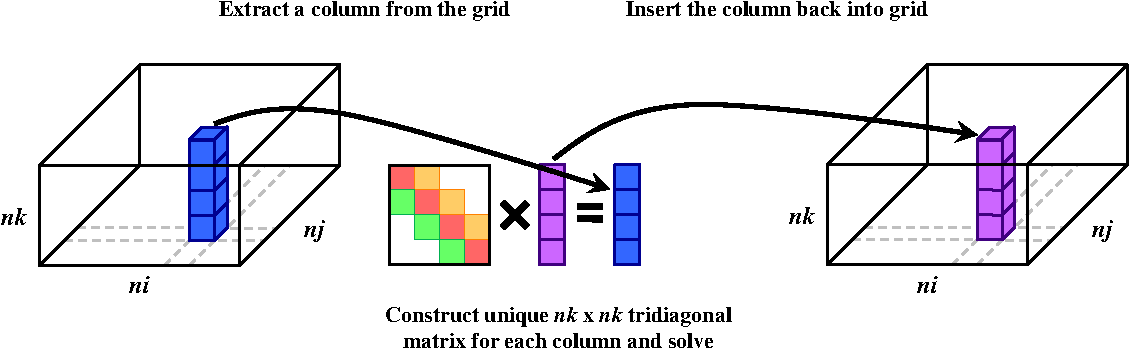
\includegraphics[width=0.95\textwidth]{figures/batching/independent_solve_diagram.pdf}
\end{figure*}

\begin{figure*}[!bth]
  \centering
  \caption{\small
    \textbf{Simultaneous Solve Strategy:} A tile of vertical columns, each 
      containing \(nk\) elements, is extracted from a \(ni \times nj \times nk\)
      3D Cartesian grid.
    All the columns in the tile are solved simultaneously, interleaving 
      the computation of individual solves.
    This approach exposes task parallelism, exhibits good data locality and
      enables vectorization in one of the horizontal dimensions (\(i\) in this
      case).
    SSTA uses this strategy.
  }
  \label{fig:impl:batching:sim_strat}
  %\vspace{1em}
  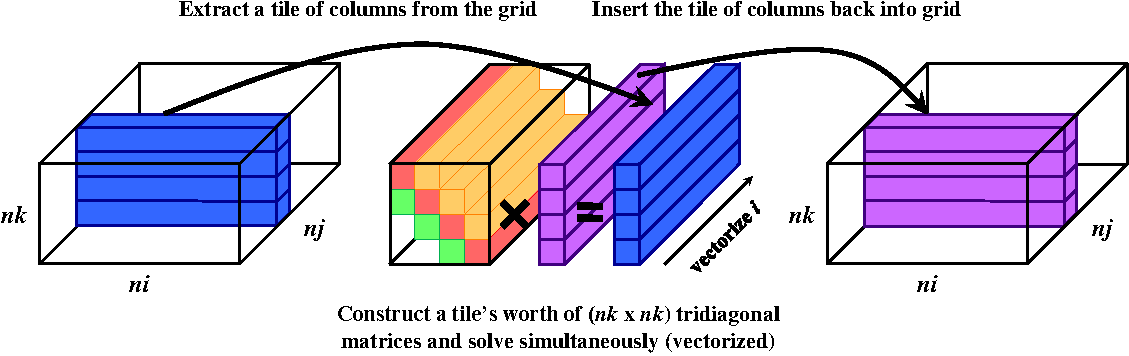
\includegraphics[width=0.95\textwidth]{figures/batching/simultaneous_solve_diagram.pdf}
\end{figure*}

We can use a simplified form of Gaussian elimination that does not require
  pivoting, known as the \textbf{Thomas algorithm} or the \textbf{tridiagonal
  matrix algorithm (TDMA)}~\cite{elem_numerical_analysis_conte}, to
  solve the type of system described by Equation \ref{eq:tridiag_system}.
The Thomas algorithm takes advantage of sparsity to be \(O(nk)\) in time, 
  and can be extended to banded matrices and LU factorizations.
It is also a significant improvement over dense Gaussian elimination,
  which is \(O(nk^3)\) in time. 
We use a formulation of the Thomas algorithm that does not require any storage
  for temporary values, but overwrites the \(b\) vector and solves for
  \(u^{s+1}\) in place (overwriting \(u^{s}\)).

The Thomas algorithm consists of two passes.  First, a \textbf{forward} pass is
  performed to \textbf{eliminate} the \(a_k\) elements:
\begin{lstlisting}
for (auto k = 1; k < nk; ++k) {
  auto const m = a[k] / b[k - 1];
  b[k] -= m * c[k - 1];
  u[k] -= m * u[k - 1];
} 
\end{lstlisting}
Then, an abbreviated form of \textbf{back substitution} is performed to obtain
  the solution:
\begin{lstlisting}
u[nk - 1] = u[nk - 1] / b[nk - 1];

for (auto k = nk - 2; k >= 0; --k) 
  u[k] = (u[k] - c[k] * u[k + 1]) / b[k];
\end{lstlisting}

The Thomas algorithm has very low
  \textbf{arithmetic intensity (AI)}~\cite{roofline}.
During the course of our work, we developed a \textbf{theoretical peak
  performance model} for the Thomas algorithm.

First, we count the number of floating point operations (FLOPs) performed.
We will consider multiplication, addition and division operations as FLOPs.
Each iteration of the forward elimination loop contains 1 division, 2
  multiplications and 2 subtractions.
This gives us a total of either \(3(nk-1)\) FLOPs on fused-multiply-add (FMA)
  architectures~\cite{intel_sw_dev_manual_2c} or 
  \(5(nk-1)\) FLOPs on non-FMA architectures.
Next, the pre-substitution operation (the assignment to \lstinline{u[nk - 1]}
  in the back substitution loop) performs a single division.
Finally, the back substitution loop performs 1 multiplication, 1
  subtraction and 1 division, adding either \(2(nk-1)\) FLOPs (FMA architectures)
  or \(3(nk-1)\) FLOPs (non-FMA architectures).
In total, this gives us either \(5nk-4\) FLOPs (FMA) or \(8nk-7\) FLOPs
  (non-FMA) for the entire Thomas algorithm.

Next, we must determine the amount of data movement that occurs in the Thomas
  algorithm.
We start by assuming that we will achieve optimal performance when
  \(a\), \(b\), \(c\) and \(u\) are cached in between the forward elimination
  loop and the back substitution loop.

The Thomas algorithm accesses four arrays, reading from all of them and writing
  to two of them (\(b\) and \(u\)).
\(b\) and \(u\) have extent \(nk\), so we store \(2nk\) elements.
\(a\) and \(c\) have extent \(nk-1\), so we load \(2(nk-1)+2nk\) elements.
In total, \(6nk-2\) elements are moved.
Assuming 8 byte elements (e.g. double precision), \(48nk-16\) bytes are moved to
  and from main memory during execution of the Thomas algorithm.

This gives us a FLOPs/byte ratio of \((5nk-4)/(48nk-16)\) (FMA) or
  \((8nk-7)/(48nk-16)\) (non-FMA).
The lower bound for arithmetic intensity is \(1/32\)
  FLOPs/byte when \(nk=1\). 
The upper bound is \(5/48\) FLOPs/byte (FMA) or \(1/6\) FLOPs/byte (non-FMA) as
  \(nk\) approaches infinity.
Based on this analysis, we can conclude that the Thomas algorithm is
  \textbf{memory-bandwidth bound}.
Thus, we use effective bandwidth, not FLOPs, as our performance metric.

We verified our analytic model by measuring hardware performance counters that
  track memory traffic with the Intel VTune Amplifier XE
  profiler~\cite{intel_vtune_amplifier}.
We found that memory bandwidth measured via hardware counters generally agreed
  with our model. 

\subsection{Batching and Vectorization}
\label{sec:impl:batching_and_parallelism}

In the applications described in \S\ref{sec:intro} we need to apply the
  Thomas algorithm to each vertical column in a \(ni \times nj \times nk\)
  3D Cartesian grid, where \(i\) and \(j\) are \textbf{horizontal dimensions}
  and \(k\) is the \textbf{vertical dimension}.
These computations are known as \textbf{vertical solves}.
Since each vertical solve is independent of the others, this is an
  embarrassingly parallel problem.
The matrix coefficients for each column depend on the problem state, so a
  unique matrix needs to be constructed before each solve.
There are two different approaches to computing these batch solves.

The most straightforward approach is to solve each column independently
  (the \textbf{independent solve strategy}; Figure~\ref{fig:impl:batching:ind_strat}).
An \(nk \times nk\) tridiagonal matrix is constructed for each vertical column,
  and then the Thomas algorithm is used to solve the linear system formed by the
  matrix and the column.
Because the vertical solves are independent, they can be executed concurrently
  via task-level parallelism.
Vectorization of the \(nk\) loop is not possible as each iteration of the loops
  in the Thomas algorithm depends on the prior iteration (e.g.
  loop-carried dependencies)~\cite{pipelined_thomas_algorithm}.
Even if it was possible to vectorize in the vertical dimension \(k\), it would
  still be undesirable to do so.
The extent of the vertical dimension is small enough in the applications
  we are concerned with - \(O(30-100)\) - that it inhibits vectorization as
  well.

The other approach is to simultaneously solve multiple columns (the
  \textbf{simultaneous solve strategy}; Figure
  \ref{fig:impl:batching:sim_strat}).
A block \(nk \times nk\) tridiagonal matrix is
  constructed for the whole grid; each block contained within the matrix is
  an \(ni \times nj\) horizontal plane.
To perform the vertical solves, we view the entire 3D grid as an
  \(nk\) block vector of \(ni \times nj\) planes and apply it to the block
  matrix.
Each step of the algorithm is applied across an entire plane.
The forward pass becomes:
\begin{lstlisting}
for (auto k = 1; k < nk; ++k)
 for (auto j = 0; j < nj; ++j)
  for (auto i = 0; i < ni; ++i) {
    auto const m = a[i][j][k] / b[i][j][k - 1];
    b[i][j][k] -= m * c[i][j][k - 1];
    u[i][j][k] -= m * u[i][j][k - 1];
  } 
\end{lstlisting}

This approach facilities both task-level parallelism and vectorization.
The grid can be tiled into smaller sub-grids, and the Thomas
  algorithm can be applied to each sub-grid independently.
Each step of the Thomas algorithm can be vectorized across the \(ni \times nj\)
  horizontal plane that it is operating on: e.g. the \(i\) or \(j\) loop in the
  above snippet can be vectorized.

The vector parallelism exposed by the simultaneous approach offers a major
  benefit over the independent approach.
It is necessary to vectorize even for a memory-bandwidth bound problem like the
  Thomas algorithm, as peak memory bandwidth cannot be achieved without
  exploiting wider vector loads and stores.

Our MKL baseline solver uses the independent solve approach, while SSTA uses
  the simultaneous solve strategy.

\subsection{Data Layout}
\label{sec:impl:data_layout}

The data layout of the 3D Cartesian grid has a huge impact on the performance
  of our solver.
Throughout the course of our research, our understanding of the impact of
  different data layouts has evolved substantially.
We have investigated three different schemes: \(ijk\), \(kji\) and \(ikj\)
  (Table~\ref{tab:impl:layout:types}).

\begin{table}[h]
\centering
% NOTE: kji AKA column-major, Fortran, left
% NOTE: ijk AKA row-major, C++, right
\caption{\textbf{Data Layouts for the 3D Cartesian Grid}}
\begin{tabular}[t]{|l|rr|r|} \hline
%%%%%%%%%%%%%%%%%%%%%%%%%%%%%%%%%%%%%%%%%%%%%%%%%%%%%%%%%%%%%%%%%%%%%%%%%%%%%%%
  \multicolumn{1}{|c|}{\multirow{2}{*}{\textbf{Name}}}
& \multicolumn{1}{ c }{\textbf{\(i\)-stride}}
& \multicolumn{1}{ c|}{\textbf{\(j\)-stride}}
& \multicolumn{1}{ c|}{\textbf{\(k\)-stride}} \\
%%%%%%%%%%%%%%%%%%%%%%%%%%%%%%%%%%%%%%%%%%%%%%%%%%%%%%%%%%%%%%%%%%%%%%%%%%%%%%%

& \multicolumn{2}{c|}{\textbf{(Horizontal)}}

& \multicolumn{1}{c|}{\textbf{(Vertical)}}   \\ \thickhline
%%%%%%%%%%%%%%%%%%%%%%%%%%%%%%%%%%%%%%%%%%%%%%%%%%%%%%%%%%%%%%%%%%%%%%%%%%%%%%%
  \(ijk\), Column-Major
& \multicolumn{1}{r|}{\(1\)}
& \multicolumn{1}{r|}{\(ni\)}
& \((ni)(nj)\)                              \\ \hline
%%%%%%%%%%%%%%%%%%%%%%%%%%%%%%%%%%%%%%%%%%%%%%%%%%%%%%%%%%%%%%%%%%%%%%%%%%%%%%%
  \(kji\), Row-Major
& \multicolumn{1}{r|}{\((nj)(nk)\)}
& \multicolumn{1}{r|}{\(nk\)}
& \(1\)                                     \\ \hline
%%%%%%%%%%%%%%%%%%%%%%%%%%%%%%%%%%%%%%%%%%%%%%%%%%%%%%%%%%%%%%%%%%%%%%%%%%%%%%%
  \(ikj\)
& \multicolumn{1}{r|}{\(1\)}
& \multicolumn{1}{r|}{\((ni)(nz)\)}
& \(ni\)                                    \\ \hline
%%%%%%%%%%%%%%%%%%%%%%%%%%%%%%%%%%%%%%%%%%%%%%%%%%%%%%%%%%%%%%%%%%%%%%%%%%%%%%%
\end{tabular}
\label{tab:impl:layout:types}
\end{table}

\begin{figure*}[!bth]
  \centering
  \caption{\small
    \textbf{Example of Different Layouts and Tiling Schemes:}
      The SSTA solver supports four layout and tiling scheme combinations.
      The figures below show how the different combinations would partition an
        \(d \times d \times e\) grid into four tiles each containing
        \((d^2/4)(e)\) elements (one tile is shown).
      With the tile-\(ij\) scheme we get \(d/2 \times d/2 \times e\) tiles,
        and with the tile-\(j\) scheme we get \(d \times d/4 \times e\) tiles.
      Different colors indicate different contiguous regions within the tile.
      Regions with similar colors have greater locality with each other. 
  }
  \label{fig:impl:tiling_schemes}
  %\vspace{1em}
  \begin{minipage}{0.49\textwidth}
    \centering
    \subfloat[
      \textbf{\(ijk\)-Layout with the Tile-\(ij\) Scheme:}
      \((d/2)(e)\) contiguous \(i\)-rows each containing \(d/2\) elements.
      This layout and tiling combination exhibits the least contiguity for the
        \(ijk\)-layout.
    ]{        
      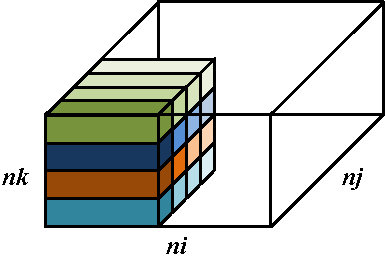
\includegraphics[width=0.70\columnwidth]{figures/tiling/ijk_layout_tile_ij_scheme_diagram.pdf}
      \label{fig:impl:tiling:ijk_tile_ij_scheme}
    }
  \end{minipage}
  \begin{minipage}{0.49\textwidth}
    \centering
    \subfloat[
      \textbf{\(ijk\)-Layout with the Tile-\(j\) Scheme:}
      \(e\) contiguous \(ij\)-planes, each containing \(d^2/4\) elements.
      This layout and tiling combination exhibits the greatest contiguity for the 
        \(ijk\)-layout.
    ]{
      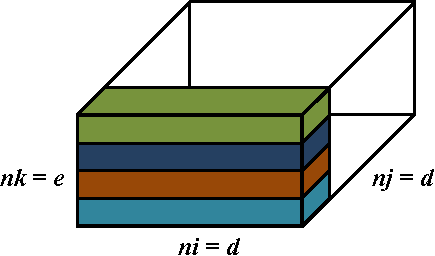
\includegraphics[width=0.70\columnwidth]{figures/tiling/ijk_layout_tile_j_scheme_diagram.pdf}
      \label{fig:impl:tiling:ijk_tile_j_scheme}
    }
  \end{minipage}
  \hspace{0em}
  \begin{minipage}{0.49\textwidth}
    \centering
    \subfloat[
      \textbf{\(ikj\)-Layout with the Tile-\(ij\) Scheme:}
      \((d/2)(e)\) contiguous \(i\)-rows each containing \(d/2\) elements.
      This layout and tiling combination exhibits the least contiguity for the
        \(ikj\)-layout.
    ]{        
      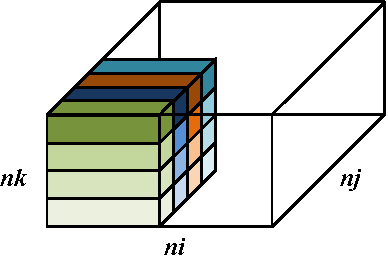
\includegraphics[width=0.70\columnwidth]{figures/tiling/ikj_layout_tile_ij_scheme_diagram.pdf}
      \label{fig:impl:tiling:ikj_tile_ij_scheme}
    }
  \end{minipage}
  \begin{minipage}{0.49\textwidth}
    \centering
    \subfloat[
      \textbf{\(ikj\)-Layout with the Tile-\(j\) Scheme:}
      One contiguous region containing \((d^2/4)(e)\) elements.
      This layout and tiling combination exhibits the greatest contiguity out of
        the four options.
    ]{
      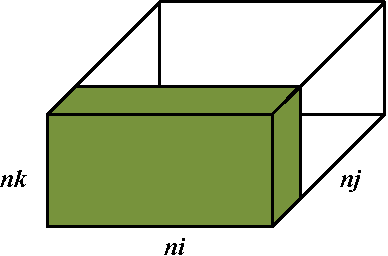
\includegraphics[width=0.70\columnwidth]{figures/tiling/ikj_layout_tile_j_scheme_diagram.pdf}
      \label{fig:impl:tiling:ikj_tile_j_scheme}
    }
  \end{minipage}
\end{figure*}

The production code that our MKL baseline solver is derived from uses the
  \(ijk\)-layout.
The vertical columns that we need to pass in to MKL as right-hand sides
  are non-contiguous, as the vertical dimension \(k\) is the dimension
  with the greatest stride.
Currently, the production codebase allocates a temporary buffer, copies data
  from the grid into the buffer, calls the LAPACK solver and then copies the
  result from the buffer back to the grid.

We have found the \(kji\)-layout to be optimal for our MKL baseline solver.
With the \(kji\)-layout, we have contiguous vertical columns that can be
  passed to MKL without temporary allocations or unnecessary copies.
We observed a noticeable performance increase from this optimization with very
  little source code change, although we have not studied the impact of this
  layout change on other components in more complex multi-kernel applications.

Our SSTA solver uses either the \(ijk\)- or \(ikj\)-layout.
SSTA vectorizes in one of the horizontal dimensions (\(i\)), so it is
  desirable to use layouts where the horizontal dimension that we are
  vectorizing is the unit stride dimension, avoiding strided vector loads.
The \(ikj\)-layout arose as an optimization to combat data locality,
  translation-lookaside buffer (TLB) and prefetching issues on Knight's
  Landing, and is described in greater detail in the next section and in
  \S\ref{sec:results:analysis}.

\subsection{Tiling}
\label{sec:impl:tiling}

To ensure good cache utilization, it is often necessary to break a larger
  grid into smaller \textbf{tiles} that better amortize nested loop overheads,
  expose greater data locality and keep data resident in a particular level of
  the cache hierarchy~\cite{cache_blocking}.
This technique is also known as \textbf{cache blocking}.
Additionally, partitioning a grid with dimensions known only at application
  initialization into fixed size tiles can provide some of the performance
  benefits of compile-time-fixed dimensions while retaining the flexibility of a
  dynamically-sized problem~\cite{kokkos}.
Tiling also provides a useful abstraction for parallel work distribution.

The production code that our MKL baseline solver is derived from is not task
  parallelized or explicitly tiled.
Since each column is solved independently, there is little opportunity to improve
  data locality and reuse via tiling (described in \S\ref{sec:results:analysis}).
Conceptually, since each column is solved independently in the production code,
  it is \textbf{effectively} tiled, albeit with a very small tile size (a single
  column).
Our MKL baseline solver is tiled solely to facilitate task parallelization.

On the other hand, tiling is very fundamental to our SSTA solver.
Our performance model (\S\ref{sec:impl:thomas_algorithm})
  is based on caching assumptions that we rely on tiling to enforce.
In particular, we assume that all four arrays (\(a\), \(b\), \(c\) and \(u\))
  remain in the cache hierarchy in between the loops of the kernel. 
If any of these four arrays need to be reloaded from main memory, the amount of
  data movement is significantly increased and the arithmetic intensity of the
  algorithm decreases dramatically.
On the platforms covered in this paper, we typically aim to fit within the L2
  cache.
While our untiled SSTA results outperform the MKL baseline results, they were
  well below the manufacturer-specified bandwidth and STREAM Triad effective
  bandwidth (Figure \ref{fig:results:percent_stream_bw}).

It is important to note the distinction between \textbf{per-array tile size}
  (e.g. the tile size for one of the four arrays) and the
  \textbf{total tile size} (e.g. the sum of the per-array tile sizes).
The total tile size is the amount of data we need to remain in cache in between
  the forward elimination loop and the back substitution loop.
Unless stated otherwise, when we refer to ``tile size'' we mean
  total tile size.

Due to the loop-carried dependencies in the Thomas algorithm and the small
  extent of \(nk\), we could not tile the vertical dimension. So, we explored
  two tiling schemes that partition the horizontal \(ij\)-plane.

The \textbf{tile-\(ij\) scheme} partitions both the \(i\) and \(j\) dimensions,
  yielding tiles with arbitrary horizontal shape consisting of contiguous
  \(i\)-rows.
The \textbf{tile-\(j\) scheme} partitions only the~\(j\) dimension, producing
  tiles consisting of contiguous \(ij\)-planes.
There is a trade-off between these two schemes, with the tile-\(ij\) scheme
  offering greater flexibility in tile size and the tile-\(j\) scheme offering
  greater contiguity. 

For example, suppose we partition a \(d \times d \times e\) \(ijk\)-layout
  grid into four tiles each containing \((d^2/4)(e)\) elements, with the
  tile-\(ij\) scheme producing
  \(d/2 \times d/2 \times e\) tiles
  (Figure~\ref{fig:impl:tiling:ijk_tile_ij_scheme})
  and the tile-\(j\) scheme producing
  \(d \times d/4 \times e\) tiles
  (Figure~\ref{fig:impl:tiling:ijk_tile_j_scheme}).
For the tile-\(ij\) scheme, tiles contain \((d/2)(e)\) contiguous
  \(i\)-rows of only \(d/2\) elements each.
For the tile-\(j\) scheme, tiles contain \(e\) contiguous \(ij\)-planes of
  \(d^2/4\) elements each.

While the tile-\(j\) scheme offers greater contiguity than the tile-\(ij\)
  scheme in this example, even the \(j\)-tiles are not a single
  contiguous memory region with the \(ijk\)-layout.
The only way to obtain completely contiguous tiles in the \(ijk\)-layout would
  be to tile the dimension with the greatest stride (\(k\)), which is is not an
  option as we never partition the small vertical dimension.

This limitation led us to the \(ikj\)-layout for the SSTA solver (see
  \S\ref{sec:results:analysis}).
With this layout, the direction of vectorization (\(i\)) is still the unit stride
  dimension, avoiding strided loads and facilitating hardware prefetching.
Additionally, the \(j\)-tiles are completely contiguous regions of memory,
  decreasing TLB pressure, increasing locality for caching and facilitating
  hardware prefetching.

Consider switching to the \(ikj\)-layout in the previous example.
The \(ij\)-tiles would be the same as before:
  \(d/2 \times d/2 \times e\) tiles consisting of \((d/2)(e)\) contiguous
  \(i\)-rows of only \(d/2\) elements each
  (Figure~\ref{fig:impl:tiling:ikj_tile_ij_scheme}).
However, the \(j\)-tiles would be one contiguous region containing all
  \((d^2/4)(e)\) elements
  (Figure~\ref{fig:impl:tiling:ikj_tile_j_scheme}).

The only notable downside to the tile-\(j\) scheme is the loss of
  flexibility in tile sizes.
The smallest tile size for the tile-\(j\) scheme is a \(d \times 1 \times e\)
  tile (an \(ik\) plane), while the smallest tile size for the
  tile-\(ij\) scheme is a \(1 \times 1 \times e\) tile (a single column).
We have not found this restriction to be problematic.

We present results from SSTA with the tile-\(j\) scheme and both the \(ijk\)-
  and \(ikj\)-layout in this paper (see \S\ref{sec:results:analysis}).

%%%%%%%%%%%%%%%%%%%%%%%%%%%%%%%%%%%%%%%%%%%%%%%%%%%%%%%%%%%%%%%%%%%%%%%%%%%%%%%
\section{Experimental Setup}
\label{sec:setup}
We developed the Tridiagonal Solve Benchmarks (TSB) suite during the course of
  our research~\cite{tsb_git}.
The TSB suite is freely available on Github under the Boost Software License,
  version 1.0.
Git tag \lstinline{ssta_paper_09_2016} contains the source code used for the
  experiments in this paper.

\subsection{Test Problem}
\label{sec:setup:test_problem}

The benchmarks in the TSB suite solve a vertical diffusion test problem on a 3D
  Cartesian grid with a time-stepping method.
Each time-step, a matrix  derived from the implicit Backward Time, Centered
  Space (BTCS) finite difference stencil with Dirichlet boundary conditions is
  solved in each vertical column. 
The diagonally-dominant tridiagonal matrix takes the following form,
  where \(D\) is a dimensionless diffusion coefficient (\(D > 0\)),
  \(\Delta \, t\) is the time step size, \(\Delta \, k\) is the vertical grid
  spacing and \(r=D \, \Delta \, t / (\Delta k)^2 \):
\begin{align*}
A = 
\begin{bmatrix}
1   & 0      &     &        & 0  \\
-r  & 1 + 2r & -r  &        &    \\
    & ...    & ... & ...    &    \\
    &        & -r  & 1 + 2r & -r \\
0   &        &     & 0      & 1
\end{bmatrix}  
\end{align*}
An identical form of the problem is initialized in every vertical column of the
  grid and a matrix is constructed for each vertical solve.

\subsection{Hardware Platforms}
\label{sec:setup:hardware_platforms}

The TSB suite currently targets x86-64 micro-architectures with SIMD vector units
  running POSIX-compliant operating systems.
The results presented in this paper were collected from both Intel Xeon and
  Xeon Phi systems.

Our two Intel Xeon platforms, Edison and Cori Phase~1, are homogeneous Cray
  supercomputers, consisting of traditional dual-socket x86-64
  nodes~\cite{nersc_systems}.
Edison features Intel Xeon E5-2695 v2 Ivy Bridge
  (IVB) processors~\cite{intel_ark_xeon_e5_2695_v2}; Cori Phase 1 has Intel
  Xeon E5-2698 v3 Haswell (HSW) processors~\cite{intel_ark_xeon_e5_2698_v3}.
Both Xeon platforms have a very similar performance profile for
  our benchmark.
In all experiments we restricted ourselves to a single socket. 

Our Xeon Phi testbed, which features Intel Xeon Phi 7210 Knight's Landing
  (KNL) processors~\cite{intel_ark_xeon_phi_7210}, is notably different from
  the two Xeon systems.
Knight's Landing is a many-core design with a 2D mesh of
  \textbf{lightweight cores} optimized for throughput and parallelism
  at the expense of increased latency and reduced complexity in other areas
  (branch prediction, out-of-order execution facilities, pipeline depth, etc).
The KNL micro-architecture has a number of novel features including on-package
  high-bandwidth MCDRAM, four hyper-threads per core and two AVX512
  vector units per core.~\cite{roofline_knl,knl_sodani}

Knight's Landing processors can be configured for different Non-Uniform Memory
  Access (NUMA) topologies.
Additionally, the MCDRAM can be configured as either programmable memory or a
  direct-mapped last-level cache~\cite{knl_sodani}.
For all experiments in this paper, we used a
  \lstinline{quadcache}~\cite{roofline_knl} configuration, where all cores 
  are in a single NUMA domain and all 16GB of MCDRAM are used as a cache.

\subsection{Toolchain}
\label{sec:setup:toolchain}

TSB is written in ISO C++14~\cite{cxx14_spec} and has no external software
  dependencies.
The code contains no vector intrinsics or assembly.
We rely entirely on the compiler vectorization engine for performant vector
  code generation, utilizing compiler directives and builtins to guide
  parallelization and vectorization, and indicate alignment, loop trip count and
  aliasing assumptions.

SSTA is task-parallelized using OpenMP \lstinline{#pragma}s~\cite{openmp_spec}.
Since the problem is embarrassingly parallel in the horizontal dimensions, it
  is easy to statically load balance.

The Intel C++ Compiler~\cite{intel_cpp_compiler} was used to compile the TSB
  suite for all of the results presented in this paper.
We used the 2017 Beta Update 2 version (\lstinline{17.0.0 20160517}).
We also used the Intel VTune Amplifier XE profiler~\cite{intel_vtune_amplifier}
  during our research.

\subsection{Statistical Considerations}
\label{sec:setup:stats}

As described in \S\ref{sec:impl:thomas_algorithm}, \textbf{effective bandwidth}
  is our primary performance metric.
We define effective bandwidth as \textbf{effective data movement} /
  \textbf{solver execution time}.

We use our theoretical peak performance model to estimate effective data
  movement.
To measure solver execution time, we record and average the wall-clock
  execution time of each time-step. 
We include OpenMP parallelization in our measurements, e.g. we time the
  \lstinline{#pragma omp for} loop instead of measuring the duration of each
  tile-iteration individually.
Thus, parallel overheads are included in our recorded execution times.

We performed each individual experiment a statistically significant number of 
  times on different nodes of our test systems.
Sample sizes varied between experiments and platforms, but were usually between
  100 to 200 independent executions per data point.
We estimated variance between different executions of the benchmark with
  identical parameters by computing sample standard deviation.
Then we constructed \textbf{95\% confidence intervals} (depicted visually with
  bars on all graphs) from the mean and sample standard deviation.

We used STREAM Triad~\cite{stream} results as a reference for peak effective
  bandwidth.
We measured a STREAM Triad bandwidth between 49.74 GB/s and 49.86 GB/s on our
  Ivy Bridge system, between 60.36 GB/s and 60.44 GB/s on our Haswell system and
  between 418.2 GB/s and 419.6 GB/s on our Knight's Landing system.

We believe there are two potential sources of non-trivial \textbf{systemic
  observational error} in our results.

First, mistakes in our analytic performance model for data movement could
  have introduced errors.
We mitigated this by verifying the model with the Intel VTune Amplifier XE
  profiler~\cite{intel_vtune_amplifier}, and we are confident in its validity.

Second, variance in the execution time of individual time-steps is not accounted
  for.
We currently average the execution time of all time-steps within a single
  run of a benchmark, but do not compute and record sample standard
  deviation as a variance estimation within the solver.
Removing this source of systemic error would be straightforward, but
  would require extending our post-processing framework to compute running 
  sample standard deviations~\cite{benchmarking_cxx_code} which we have not
  yet implemented.

%%%%%%%%%%%%%%%%%%%%%%%%%%%%%%%%%%%%%%%%%%%%%%%%%%%%%%%%%%%%%%%%%%%%%%%%%%%%%%%
\section{Results}
\label{sec:results}

\begin{figure*}[!bth]
  \centering
  \caption{\small
    \textbf{SSTA Effective Bandwidth vs. Total Tile Size:}
    The results of a parameter sweep on our two Intel Xeon platforms
      demonstrating the effect of total tile size on the performance of the
      SSTA solver is shown below (MKL baseline and STREAM Triad results shown as
      lower- and upper-bounds).
    The \(ikj\)-layout, which exhibits better contiguity and memory access
      patterns, performs better at smaller tile sizes, although the best
      \(ikj\)-layout result does not outperform the best \(ijk\)-layout result
      on these platforms.
    Performance degrades for tile sizes that exceed L3 capacity per core.
    Both SSTA variants substantially outperform the MKL baseline results and 
      reach \textapprox 90\% of STREAM Triad effective bandwidth with optimal 
      tile sizes.
    Results are shown with 95\% confidence (see \S\ref{sec:setup:stats}).
  }
  \label{fig:results:bw_vs_tile_size_xeon}
  %\vspace{1em}
  \begin{minipage}{0.49\textwidth}
    \subfloat[
      \textbf{Ivy Bridge}
    ]{        
      \includegraphics[width=0.99\columnwidth]{figures/results/effective_bandwidth_vs_total_tile_size_edison_ivb_e5_2695_v2_1socket_graph.pdf}
      \label{fig:results:bw_vs_tile_size_ivb}
    }
  \end{minipage}
  \begin{minipage}{0.49\textwidth}
    \subfloat[
      \textbf{Haswell}
    ]{
      \includegraphics[width=0.99\columnwidth]{figures/results/effective_bandwidth_vs_total_tile_size_cori_hsw_e5_2698_v3_1socket_graph.pdf}
      \label{fig:results:bw_vs_tile_size_hsw}
    }
  \end{minipage}
\end{figure*}

\begin{figure}[!h]
  \centering
  \caption{\small
    \textbf{SSTA Effective Bandwidth vs. Total Tile Size (Knight's Landing):}
    Shown below are the results of a parameter sweep on our Intel Xeon Phi
      Knight's Landing platform showing the effect of data layout and total
      tile size on the performance of the SSTA solver.
    MKL baseline (lower-bound) and STREAM Triad (upper-bound) results are shown
      for reference.
    \(ijk\)-layout performance is hampered by poor data contiguity that incurs
      expensive TLB and hardware prefetching penalties on Knight's Landing.
    This effect is amplified at smaller tile sizes.
    The best \(ikj\)-layout result has between 91 GB/s and 109 GB/s higher
      effective bandwidth than the best \(ijk\)-layout result, and reaches
      between 88\% and 92\% of STREAM Triad performance.
    Results are shown with 95\% confidence (see \S\ref{sec:setup:stats}).
  }
  \label{fig:results:bw_vs_tile_size_knl}
  \includegraphics[width=0.95\columnwidth]{figures/results/effective_bandwidth_vs_total_tile_size_carl_knl_7210_1socket_graph.pdf}
\end{figure}

\begin{figure}[!h]
  \centering
  \caption{\small
    \textbf{Percentage of STREAM Triad Effective Bandwidth Attained by SSTA:}
    Across all three micro-architectures, the SSTA solver with an optimal total
      tile size improves performance substantially over the MKL baseline, and
      achieves \textapprox 90\% of STREAM Triad effective bandwidth.
    Although untiled SSTA results beat the MKL solver, tiling contributes
      significantly to overall performance: between 35.9\% and 36.1\% on 
      Ivy Bridge, between 34.22\% and 35.38\% on Haswell and between 24\% and
      26\% on Knight's Landing.
    Between 21\% and 25\% of STREAM performance attained is attributed to the
      switch to the \(ikj\)-layout on Knight's Landing. 
    Results are shown with 95\% confidence (see \S\ref{sec:setup:stats}).
  }
  \label{fig:results:percent_stream_bw}
  \includegraphics[width=0.95\columnwidth]{figures/results/percentage_of_stream_bw_attained_histogram.pdf}
\end{figure}

% Hypothesis 1.1: SSTA can outperform legacy solver
% Hypothesis 1.2: SSTA can efficiently utilize memory bandwidth 
% Prediction 1.1 and Prediction 1.2 follow naturally 
We developed SSTA to replace the MKL-based vertical column solver in our
  production climate application because we believed better vectorization and
  data movement could be achieved by solving multiple vertical columns
  \textbf{simultaneously}.
% Hypothesis 2: SSTA will be highly sensitive to data layout changes and total
% tile size and will achieve optimal performance for a particular tile size
% that balances reuse/locality/amortization.
We also theorized that such a solver would be highly sensitive to
  \textbf{data layout changes} and
  \textbf{total tile size} (\S\ref{sec:impl:tiling}).

Parallel application performance is often driven by parameters such as 
  tile size, which control the amount of work in each parallel task.
In memory-bandwidth bound applications, data layout and tiling can be
  especially important as they not only influence the amount of task- and
  vector-parallelism exposed but also the working set size and degree of cached
  data reuse in each individual task.
We anticipated that we would need to study the effect of different data layouts
  and tile sizes in order to understand the performance of our new solver.
The first step was to determine the \textbf{optimal total tile size} for the 
  different solver variants in the TSB suite.

We conducted a parameter sweep of total tile size on our Xeon and Xeon Phi 
  platforms.
We predicted that we would see the following: 
\begin{itemize}
% Prediction 2.1: The MKL solver doesn't care about tile size, excluding
% SLOW effects.
\item The MKL baseline solver would be insensitive to total tile size, excluding
  extremely small (high overhead) and extremely large (insufficient parallelism)
  tile sizes, since it solves each column independently and thus cannot exploit
  vector instructions and data locality like the SSTA solver does.
% Prediction 2.2: Total tile sizes which fit in the L1D will be too small to be
% feasible.
\item Total tile sizes small enough to fit into the L1D cache would not be
  feasible because the overheads of loops and parallelization would be too great
  relative to the execution time of useful work per inner-loop iteration.
These tile sizes would either require vertical extents below the sizes 
  we are interested in (\(nk < 16\)) or horizontal
  extents too small to vectorize efficiently (\(ni < 16\)).
% Prediction 2.3: Optimal total tile size will be in between L1D capacity and
% L2 capacity.
\item The optimal total tile size would fit into the L2 cache, but not the L1D,
  since the L2 is the fastest cache that has the capacity to contain a
  feasible tile size.
% Prediction 2.4: Performance drops as total tile size crosses cache capacity
% boundaries, excluding L1D.
\item Excluding the L1D, as we move from a tile size that fits into the
  capacity of a particular cache to a tile size that does not, we should see a
  drop in effective bandwidth.
On the Xeon platforms, the boundaries are L2 \(\rightarrow\) L3 and L3
  \(\rightarrow\) DRAM (main memory).
On Knight's Landing, the boundaries are L2 \(\rightarrow\) MCDRAM cache and
  MCDRAM cache \(\rightarrow\) DRAM (main memory).
\end{itemize}
Note that when a total tile size is exactly equal to a particular cache
  capacity, we claim that it will not fit into that cache.

The results of this parameter sweep for both the \(ijk\)- and \(ikj\)-layout are
  shown in Figure~\ref{fig:results:bw_vs_tile_size_ivb} (Ivy Bridge),
  Figure~\ref{fig:results:bw_vs_tile_size_hsw} (Haswell) and
  Figure~\ref{fig:results:bw_vs_tile_size_knl} (Knight's Landing).
Results from the TSB suite's MKL baseline solver are shown as a lower bound,
  and STREAM Triad results are shown as an upper bound. 
A \(32 \times 147456 \times 32\) grid of double precision floating point values
  was used on all platforms (4.5GB in total for \(a\), \(b\), \(c\) and \(u\)).
All results were run on a full socket, with one application-thread bound to each
  core.

\subsection{Analysis}
\label{sec:results:analysis}

% Analysis of Prediction 2.2: The MKL solver doesn't care about tile size,
% excluding SLOW effects.
We found that the MKL baseline solver was largely insensitive to tile size, as
  predicted.
Across the range of total tile sizes we tested, we did not observe performance
  variation that was statistically significant enough to distinguish it from
  random observational error, which is what we anticipated.

% Analysis of Prediction 2.2: Total tile sizes which fit in the L1D will be too
% small to be feasible.
As we predicted, total tile sizes small enough to fit into the L1D cache were
  impractical on all platforms.
% Math for exploring tile extents that might fit into L1D
% nj=(32KB*1/2*1/4*1/sizeof(double))*(1/nk)*(1/ni)
%          ^^^ ^^^
%           1   2
% 1: reasonable target working set size 
% 2: # of arrays
We would have to either reduce the vertical extent or the horizontal
  extent \(ni\) to generate a tile size small enough to fit into the 32KB L1D
  with the tile-\(j\) scheme.
We ran preliminary experiments with \(ni=16\) (not shown) to observe the effect
  of 16KB tile sizes.
The results indicated that tile sizes smaller than 32KB performed worse for both
  the \(ijk\)- and \(ikj\)-layouts on all platforms.
At \(ni=16\), the trip count on some of the loops in SSTA is so small that the
  compiler cannot perform as much unrolling post-vectorization as it would for
  larger \(i\) extents.

% Analysis of Prediction 2.3: Optimal total tile size will be in between L1D
% capacity and L2 capacity.

% ijk Paragraph 1
On Knight's Landing, the optimal total tile size for the SSTA \(ijk\)-layout
  variant is 128KB, which is small enough to fit within the L2 but too large
  for the L1D. 
On Ivy Bridge and Haswell, the optimal total tile size for the \(ijk\)-layout 
  is 256KB, which is too large for the L2.
% Roughly 0.16 GB/s gap between the bottom of the 256KB result and the top of
% the next best on Ivy Bridge, roughly equivalent between the 256KB result and
% the next best on Haswell (0.02 GB/s overlap)
While it is difficult to distinguish between the 128KB, 256KB and 512KB results
  in Figures~\ref{fig:results:bw_vs_tile_size_ivb} and~\ref{fig:results:bw_vs_tile_size_hsw}
  because the magnitude of the difference is relatively small, the confidence
  intervals do not overlap and the trend of the dataset supports our conclusion.

% ijk Paragraph 2
We were intrigued to find that, contrary to our predictions, the optimal total
  tile size for the \(ijk\)-layout on the Xeon platforms was too large to fit
  within the L2.
Additionally, while the optimal total tile size for the \(ijk\)-layout on
  Knight's Landing would fit within the L2 cache, performance was not as close to
  peak as it was on the Xeon platforms (see Table~\ref{tab:results:summary}).

Profiling indicated that the SSTA \(ijk\)-layout variant experienced a high
  number of L1 DTLB store misses.
As we decreased total tile size, we observed progressively worse TLB performance
  in our profiling traces.
We determined this was due to the lack of fully contiguous tiles in the
  \(ijk\)-layout (see \S\ref{sec:impl:tiling}). 
As the tile size is decreased, the size of each contiguous
  plane decreases and the frequency of non-contiguous jumps through memory
  increases, negatively impacting TLB, cache and hardware prefetching performance,
  especially on Knight's Landing (See
  Figure~\ref{fig:results:bw_vs_tile_size_knl}).

% ijk Paragraph 3
We conducted a parameter sweep with the SSTA \(ijk\)-variant and a smaller
  vertical extent (\(nk = 16\), not shown) to further verify the cause of this
  issue.
With fewer vertical levels, the number of contiguous regions for each tile size
  would be decreased and the size of each contiguous region would be increased,
  improving contiguity.
We observed performance improvements with \(nk = 16\); on Knight's Landing
  the impact was significant.

% ijk Paragraph 4 (motivation to develop ikj) 
The poor performance of the \(ijk\)-layout on Knight's Landing led us to
  develop the \(ikj\)-layout variant of SSTA described in
  \S\ref{sec:impl:data_layout} and \S\ref{sec:impl:tiling}.
The optimal total tile size for the \(ikj\)-layout was 32KB on all three
  platforms.
On the Xeon platforms, the best \(ikj\)-layout result does not outperform the
  best \(ijk\)-layout result, although the \(ikj\)-layout variant does perform
  better than the \(ijk\)-layout variant at smaller tile sizes.
However, on Knight's Landing the best \(ikj\)-layout result achieves
  between 91 GB/s and 109 GB/s higher effective bandwidth than the best
  \(ijk\)-layout result (see Table~\ref{tab:results:summary}), a significant
  improvement.

\begin{table*}[t]
  \centering
  \caption{
    % AKA supertable
    \textbf{Summary of SSTA Performance Results:} 
    SSTA outperforms the MKL baseline solver on all of our test platforms. SSTA
    achieves a \textapprox \(2x\) speedup over the MKL solver on our Xeon
    platforms, a \textapprox \(12x\) speedup on Knight's Landing, and attains
    \textapprox 90\% of STREAM Triad effective bandwidth on all three platforms.
    All measurements are reported with 95\% confidence
    (see \S\ref{sec:setup:stats}).
  }
  \label{tab:results:summary}
  %\vspace{1em}
  %%%%%%%%%%%%%%%%%%%%%%%%%%%%%%%%%%%%%%%%%%%%%%%%%%%%%%%%%%%%%%%%%%%%%%%%%%%%%
  \begin{tabular}{|l|l|l|l|l|}\hline
    %%%%%%%%%%%%%%%%%%%%%%%%%%%%%%%%%%%%%%%%%%%%%%%%%%%%%%%%%%%%%%%%%%%%%%%%%%%
      \multicolumn{1}{|c|}{\multirow{2}{*}{\textbf{Solver}}}
    & \multicolumn{1}{ c|}{\textbf{Optimal Total}}
    & \multicolumn{1}{ c|}{\textbf{Effective Bandwidth}}
    & \multicolumn{1}{ c|}{\textbf{Percentage of STREAM}}
    & \multicolumn{1}{ c|}{\multirow{2}{*}{\textbf{Speedup vs. MKL}}} \\
    %%%%%%%%%%%%%%%%%%%%%%%%%%%%%%%%%%%%%%%%%%%%%%%%%%%%%%%%%%%%%%%%%%%%%%%%%%%

    & \multicolumn{1}{ c|}{\textbf{Tile Size}}
    & \multicolumn{1}{ c|}{\textbf{Bandwidth}}
    & \multicolumn{1}{ c|}{\textbf{TRIAD Bandwidth}}
    & \\ \hline
    %%%%%%%%%%%%%%%%%%%%%%%%%%%%%%%%%%%%%%%%%%%%%%%%%%%%%%%%%%%%%%%%%%%%%%%%%%%
    \multicolumn{5}{c}{\rule{0pt}{2.25ex} \textbf{Ivy Bridge}}        \\ \hline \thickhline
    % BW, Ivy Bridge MKL kji tw_sweep tw=64 results + sig figs
    % % STREAM, Ivy Bridge MKL kji histogram tw=64 results + sig figs
    MKL \(kji\)-layout  &    Any & \, \(22.49 \pm 0.003\) GB/s &\(45.2 \pm 0.05\) \% & \, \, \(1\) \;\, \(x\)        \\ \hline
    % BW, Ivy Bridge SSTA ijk tw_sweep tw=8 results + sig figs 
    % % STREAM, Ivy Bridge SSTA ijk histogram tw=8 results + sig figs
    SSTA \(ijk\)-layout & 256 KB & \, \(44.0 \; \; \pm 0.07\) \, GB/s &\(90 \; \; \; \, \pm 0.1\) \, \%    & \, \textapprox \(2\) \;\, \(x\)   \\ \hline
    % BW, Ivy Bridge SSTA ikj tw_sweep tw=1 results + sig figs 
    % % STREAM, Ivy Bridge SSTA ijk PAPER tw=1 results + sig figs
    SSTA \(ikj\)-layout & \, 32 KB & \, \(43.0 \; \; \pm 0.07\) \, GB/s &\(87 \; \; \; \, \pm 0.2\) \, \%    & \, \textapprox \(1.9\) \(x\) \\ \hline
    
    \multicolumn{5}{c}{\rule{0pt}{2.25ex} \textbf{Haswell}}           \\ \hline \thickhline
    % BW, Haswell MKL kji tw_sweep tw=64 results + sig figs
    % % STREAM, Haswell MKL kji histogram tw=64 results + sig figs
    MKL \(kji\)-layout  &   Any & \, \(31.65 \pm 0.006\) GB/s & \(52.4 \pm 0.04\) \% & \, \, \(1\) \;\, \(x\)        \\ \hline
    % BW, Haswell SSTA ijk tw_sweep tw=8 results + sig figs 
    % % STREAM, Haswell SSTA ijk histogram tw=8 results + sig figs
    SSTA \(ijk\)-layout & 256 KB & \, \(54.3 \; \; \pm 0.01\) \, GB/s & \(90.0 \pm 0.07\) \% & \, \textapprox \(1.7\) \(x\) \\ \hline
    % BW, Haswell SSTA ikj tw_sweep tw=1 results + sig figs 
    % % STREAM, Haswell SSTA ijk PAPER tw=8 results + sig figs
    SSTA \(ikj\)-layout & \, 32 KB & \, \(54.2 \; \; \pm 0.01\) \, GB/s & \(89.7 \pm 0.06\) \% & \, \textapprox \(1.7\) \(x\) \\ \hline

    \multicolumn{5}{c}{\rule{0pt}{2.25ex} \textbf{Knight's Landing}}  \\ \hline \thickhline
    % BW, Knight's Landing MKL kji tw_sweep tw=64 results + sig figs
    % % STREAM, Knight's Landing MKL kji histogram tw=64 results + sig figs
    MKL \(kji\)-layout  &   Any & \, \(32 \quad \; \pm 0.2\) \quad GB/s &\, \(7.6 \pm 0.04\) \% & \, \, \(1\) \;\, \(x\)               \\ \hline
    % BW, Knight's Landing SSTA ijk tw_sweep tw=4 results + sig figs
    % % STREAM, Knight's Landing SSTA ijk histogram tw=4 results + sig figs
    SSTA \(ijk\)-layout & 128 KB &  \(280 \quad \; \pm 5\) \; \; \, GB/s &\(66 \; \; \; \, \pm 1\) \; \; \%     & \, \textapprox \(9\) \;\, \(x\)          \\ \hline
    % BW, Knight's Landing SSTA ikj tw_sweep tw=1 results + sig figs
    % % STREAM, Knight's Landing SSTA ikj histogram tw=1 results + sig figs
    SSTA \(ikj\)-layout & \, 32 KB &  \(370 \quad \; \pm 6\) \; \; \, GB/s &\(90 \; \; \; \, \pm 2\) \; \; \%     & \textapprox \(12\) \;\, \(x\)         \\ \hline
    %%%%%%%%%%%%%%%%%%%%%%%%%%%%%%%%%%%%%%%%%%%%%%%%%%%%%%%%%%%%%%%%%%%%%%%%%%%%
  \end{tabular}
\end{table*}

% Summary 
Our prediction that the optimal total tile size would be larger than L1D
  capacity but smaller than L2 capacity held for the \(ikj\)-layout on all
  platforms and also for the \(ijk\)-layout on Knight's Landing.
For the \(ijk\)-layout on the Xeon platforms, the optimal total tile size was
  too large to fit into the L2.
We believe the difference between optimal total tile sizes on the Xeon
  platforms and Knight's Landing is due to the lack of a traditional L3 cache
  on the latter, making the performance penalty greater for L2 misses.
We can draw the conclusion that, for the platforms surveyed, the optimal total
  tile size for the \(ijk\)-layout is large enough to reside in the
  last-level associative on-die cache (the L3 on the Xeon platforms and the L2
  on Knight's Landing).

% Prediction 2.4: Performance drops as total tile size crosses cache capacity
% boundaries, excluding L1D.
The total tile size parameter sweep mostly supports our prediction that
  performance drops when going from tile sizes that fit into a particular cache
  to tile sizes that do not.
We see no such decrease at the L2 capacity boundary on the Xeon platforms, but
  we do see a drop when the tile size exceeds L3 capacity per core.
On Knight's Landing, we see a drop as we cross the L2 capacity boundary.
We posit that a modified version of our prediction is more accurate; as we move
  from a tile size that will fit into the last-level associative on-die cache
  to a tile size that will not, there is a drop in SSTA's effective bandwidth.

%%%%%%%%%%%%%%%%%%%%%%%%%%%%%%%%%%%%%%%%%%%%%%%%%%%%%%%%%%%%%%%%%%%%%%%%%%%%%%%
\section{Conclusion}
\label{sec:conclusion}

% Analysis of Prediction 1.1 (can outperform legacy solver)
% Analysis of Prediction 1.2 (can efficiently utilize memory bandwidth)

We introduced the Simultaneous Streaming Thomas Algorithm (SSTA) solver, which
  can efficiently solve many small tridiagonal matrix systems simultaneously, 
  and addresses a performance bottleneck
  that arises in a number of scientific application domains.
We have demonstrated the impact of different tiling schemes, tile sizes
  and data layouts, and how they interact with the memory sub-system.

We found that the \(ijk\)-layout version of SSTA provides the best performance
  on Xeon platforms with a total tile size that is small enough to fit into 
  the L3 cache but is too large to fit in the L2.
On Knight's Landing, the \(ikj\)-layout yields the best performance with a
  tile size that is small enough to fit in the L2.

Our results are summarized in Table~\ref{tab:results:summary}.
They show that SSTA is a highly efficient solver capable of achieving 90\%
  of STREAM Triad bandwidth on Intel Xeon and Xeon Phi systems, including the new
  Knight's Landing micro-architecture.
Our algorithm is a substantial improvement over the MKL-based \(kji\)-layout
  baseline solver; it is \textapprox \(2x\) faster on Xeon platforms and
  \textapprox \(12x\) faster on Knight's Landing.

\section{Future Work}
\label{sec:future}

There are also a number of optimizations that we developed for the SSTA
  solver but have not presented here. 
The version of the TSB suite described in this paper uses what we refer to as
  the \textbf{full-grid scheme}, where the tridiagonal matrix is built and
  stored for all vertical columns.
The alternative \textbf{rolling-grid scheme} builds the matrix on the fly in
  a tile-sized \(a\), \(b\) and \(c\).
In addition to offering storage savings, we believe the rolling-grid scheme
  will further improve data locality and hardware prefetching performance as the
  storage for the matrix will be reused for all tiles that a core executes
  (each column's matrix may still be different).
%This would be especially appropriate for non-linear solvers, where the 
%  matrix needs to be updated every iteration.
Further research is also needed to explore smaller total tile sizes, as well as
  the tile-\(ij\) scheme, as it may be beneficial to production applications that
  are willing to accept some performance trade-off for increased flexibility in
  the extent of the horizontal dimension \(i\).

%We developed two optimizations which reduced the number of floating point
%  divisions and/or reciprocal estimates that are performed by the SSTA solver. 
%The first, the \textbf{cached-divide} optimization, reformulates the Thomas 
%  algorithm to remove the division operation from the back substitution loop by
%  storing the reciprocal of the temporary value that is written to the array
%  \(b\) in the forward elimination loop instead of storing the temporary value
%  itself.
%The second optimization is specific to Intel AVX and AVX2 systems like the Xeon
%  test platforms used in this paper.
%Such platforms provide a single-precision vector reciprocal instruction
%  (RCPPS) but no corresponding double-precision
%  operation~\cite{intel_opt_manual}.
%We developed a double-precision vector division implementation,
%  \textbf{NR-RCPPS division}, which converts to single precision, performs an
%  RCPPS operation, converts back to double precision and then performs Newton
%  Raphson iterations.
%While we found both optimizations to be beneficial in serial, they decreased
%  performance if combined together and had little impact in parallel.


We would like to extend the range of hardware platforms and configurations in
  future experiments.
On Knight's Landing, further effort is needed to study the trade-off between
  utilizing MCDRAM as a cache versus programmable memory.
We are also interested in testing SSTA on SIMT GPGPU architectures.

There are also a number of related numerical problems that we believe could be
  addressed by some of the techniques we describe in this paper.
The algorithm could be extended to include matrix assembly
  based on solution values and put inside a fully non-linear iteration
  with a Jacobian calculation, such as those used in Newton iterations.
The challenge here is that some vertical columns may converge faster than
  others, which may require vector masking or scalar iterative refinement.
Opportunities to extend the algorithm to banded or other sparse matrices
  and incomplete LU-type algorithms are straight-forward for diagonally-dominant
  cases, but pivoting has the potential to hinder vectorization and memory
  access patterns.

Finally, more complex multi-kernel applications integrate multiple solvers and
  computational phases, such as traditional finite difference
  stencil operations and time integration algorithms. 
We will have to explore the performance trade-offs between
  the \(ijk\)-, \(kji\)- and \(ikj\)-layouts in these applications.
% Closer.

Our efforts in the immediate future will revolve around research into those
  trade-offs and the integration of SSTA into our production software.

\section*{Acknowledgments}
\label{sec:ack}
This material is based upon work supported by the U.S. Department of Energy
  Office of Science's Scientific Discovery through Advanced Computing (SciDAC)
  program and the Intel Parallel Computing Center (IPCC) at Lawrence Berkeley
  National Laboratory (LBNL).
Resources at the National Energy Research Scientific Computing Center (NERSC),
  which is supported by the U.S. Department of Energy Office of Science's
  Advanced Scientific Computing Research (ASCR) program (contract
  DE-AC02-05CH11231), were used to produce this work.

Our thanks to Cy Chan for providing early feedback and identifying a serious
  error in Figure \ref{fig:impl:tiling:ikj_tile_ij_scheme}.

\newpage

\bibliographystyle{IEEEtran}
\bibliography{ssta}

\end{document}

